
\documentclass{sig-alternate}
\usepackage{hyperref}
\begin{document}
\conferenceinfo{WOODSTOCK}{'97 El Paso, Texas USA}
%\CopyrightYear{2007} % Allows default copyright year (20XX) to be over-ridden - IF NEED BE.
%\crdata{0-12345-67-8/90/01}  % Allows default copyright data (0-89791-88-6/97/05) to be over-ridden - IF NEED BE.
% --- End of Author Metadata ---
\title{Web Interpreter Negative Testing with Evolutionary Methods}

\numberofauthors{3} 

\author{
\alignauthor
Spandan Veggalam\\
       \affaddr{IIIT-Hyderabad}\\
       \affaddr{Hyderabad,India}\\
       \email{
       veggalam.s@reseach.iiit.ac.in}
\and
% 3rd. author
\alignauthor
Sanjay Rawat\\
       \affaddr{IIIT-Hyderabad}\\
       \affaddr{Hyderabad,India}\\
       \email{sanjay.rawat@iiit.ac.in}
}

\maketitle

\begin{abstract}
Fuzzing is an automated black box testing used for finding security vulnerabilities in the software. Fuzzing ensure that product doesn't fail with indigestible input and tests its correctness. Fuzz testing randomly generates well formed inputs and tests the program with the resulting data. \\ \indent In this paper we use evolutionary techniques in generating inputs to test the interpreters. Fuzzed input must be syntactically valid program, which is an elementary condition of an Interpreter. On the other hand Interpreter accepts only semantically valid program, and fuzzed input program must trigger exceptional  of Interpreter such as crashes, memory leaks, failing assertions.\\
\indent In this paper we propose \textit{GEInterpreterFuzz} an evolutionary approach to generate input code fragments and fuzz the Interpreter. GEInterpreterFuzz is language independent approach generates code fragments based on language grammar specifications using grammatical evolution techniques. 
\end{abstract}

\category{}{Security and Privacy}{Systems Security}[Vulnerability detection]
\terms{Security Testing}
\keywords{Security, Fuzzing, JavaScript, Grammatical Evolution, Evolutionary Algorithm, 
Artificial Intelligence, Web Applications, Interpreters}

\section{Introduction}
\indent Software security is essential dimension for a software. Web browser, because they are front end for networks and computer systems, are some of primary applications for security attacks, data breaches and privacy breaches. Moreover browsers, being the favourite client web interface, are becoming more and more sophisticated in terms of content they can render. Nowadays, they include interpreters
for languages such as JavaScript (JS), SVG, PDF, XSLT. It is well recognized that Interpreters can be exploited to launch browser based security attacks. For example over the years JavaScript is responsible for several vulnerabilities. We look at such attacks in the following perspective:
\begin{enumerate}
\item Some attacks exploit the vulnerabilities that arise due to the way information is extracted, parsed, stored, manipulated and communicated:
\\e.g., Cross Site Scripting
\item Other exploit vulnerabilities in the software's that browser makes use of script engines, plug-ins, etc., Often, these are low-level vulnerabilities
\\e.g., memory corruptions, assertion failures, uncommon behaviours etc.
\end{enumerate}
\indent The Web has proved to be the main medium for information sharing. In the recent past, there have been numerous studies, techniques, and tools proposed to address the security issues related to above mentioned point 1. However, in the context of web related vulnerabilities particularly browsers and interpreters, not much has been investigated in the direction of the above mentioned point 2. As a result, recently, there have been many bugs uncovered in browser-run software's: e.g. Firefox JS engine.\\
\indent Fuzz testing is a useful approach for finding vulnerabilities in softwares. One of its variants, evolutionary fuzzing, turned out to be a useful smart fuzzing method. These methods make use of evolutionary computing approaches to automatically generate inputs that exhibit vulnerabilities.\\
\indent Fuzzed input must be syntactically valid otherwise interpreter simply discards the input as invalid. Therefore input must be generated making use of knowledge about target language. Assuming JavaScript interpreter to be target, fuzzed input must follow the syntax rules of JavaScript. Otherwise JavaScript interpreter discards the inputs. For this JavaScript language grammar is used to generate code fragments. With built-in language grammar valid data can be modelled. Both language dependent and independent fuzzer can be built with some additional knowledge of a specific language. \textit{jsfunfuzz} is popular fuzzer for Mozilla's JavaScript engine. This is an example for language dependent fuzzer. Another fuzzer \textit{Langfuzz} is an example of language independent fuzzer generates syntactically valid code fragments. With the motivation from this language independent fuzzer can we map langfuzz approach to Genetic programming paradigm?\\
\indent In this paper we will introduce a new framework called \textit{GEInterpreterFuzz}, that generates code fragments using Grammatical Evolution methods (particular form of Genetic Programming), thereby allows black box fuzzing of the Interpreters. GEInterpreterFuzz takes context free grammar as input, for instance given JavaScript grammar it generates JavaScript programs; uses grammar to learn code fragments from the code base. Given a test suite, GEInterpreterFuzz performs standard Gentic Algorithm  operations; crossover and mutations on the input code fragments and uses learnt code fragments for replacements - Grammatical Evolution brings transparency on making decision, inspired by biological evolution. It follows Darwin's theory of evolution and selects programs with high fitness. Here, Fitness function favours  the program which are uncommon enough and likely to trigger interpreter exceptional behaviors and are selected for fuzzing. Grammatical Evolution approach is appropriate at generating code, and likely to produce diverse code fragments
\begin{figure*}
\centering
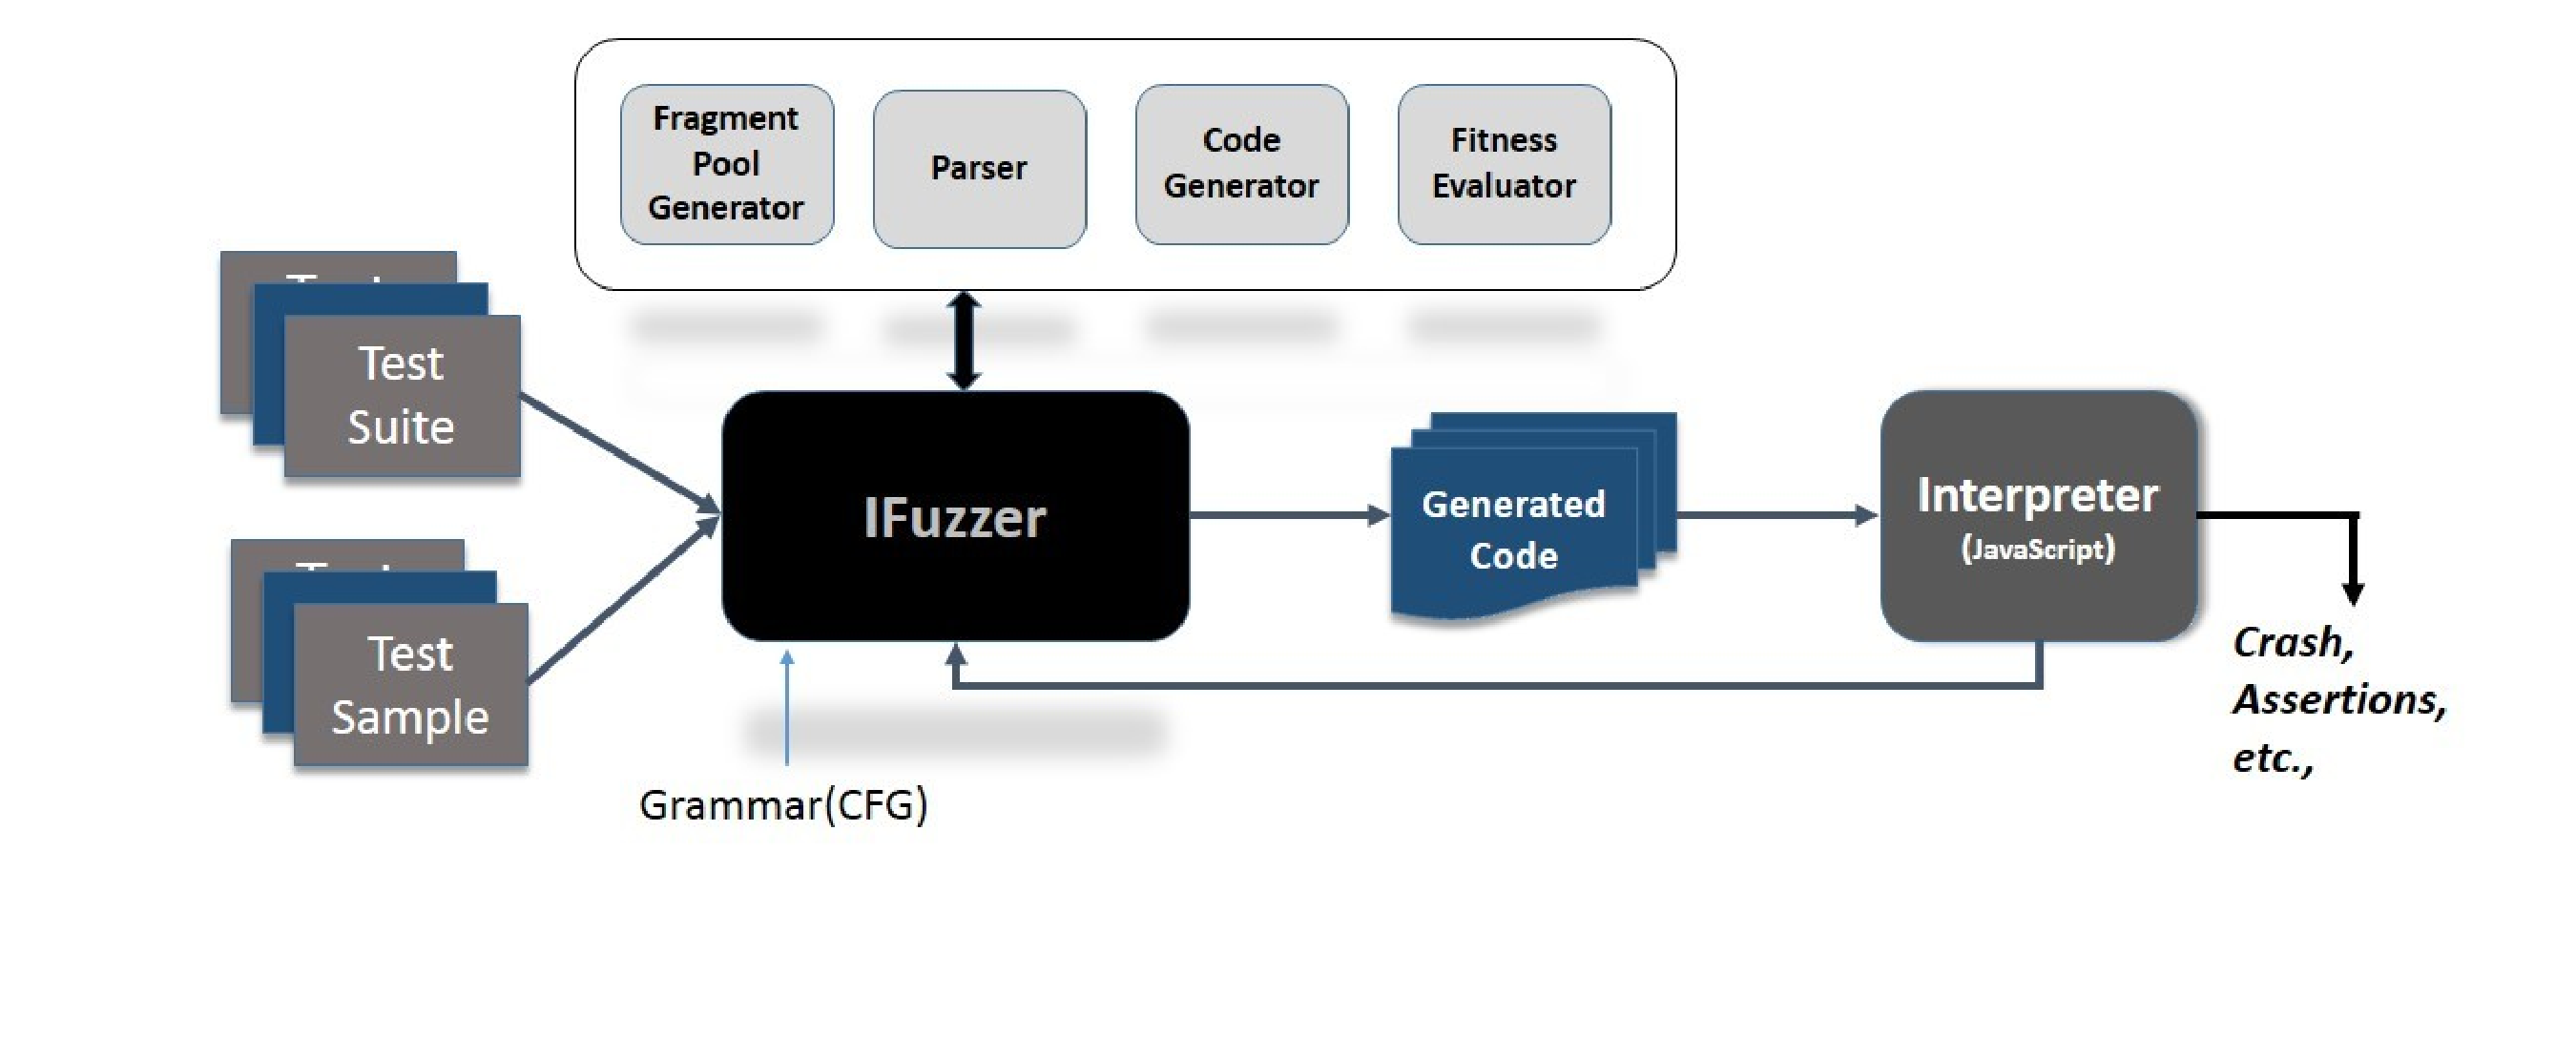
\epsfig{file=process.eps, height= 2.5in, width=6.5in}
\caption{Overview of GEInterpreterFuzz Approach.}
\label{fig1}
\end{figure*}
\\\indent  Figure \ref{fig1} describes the overview of GEInterpreterFuzz which takes test suite, language grammar and sample code as input. Language grammar is used to parse the program. Parser uses language grammar to parse the program and generates XML object as abstract syntax representation. Fragment pool of code fragments formed by parsing each input file from sample codes. Test suite itself can be used as sample codes. GEInterpreterFuzz generates new code fragments by performing genetic operations on the test suite. 
\\Remaining paper explains the code generation process and fuzzing process. ~\autoref{sec:bk} presents the motivation for choosing Grammatical Evolution for code generation. In ~\autoref{sec:GEIF} we describe the methods involved in code generation process. Implementation of GEInterpreterFuzz is discussed in ~\autoref{sec:impl}.
\section{Motivation} \label{sec:bk}

\subsection{Terminology}
\indent In the following sections we make use of following terminology.
\begin{enumerate}
\item{\textbf{Interpreter.}} In this paper the term \textit{"Interpreter"} is software system that executes input program. This translates code from one form to other form during execution. 
\item{\textbf{Genotype.}} In this paper the term \textit{"Genotype"} refers to the structural representation of the program which is operated on by crossover and mutation
\item{\textbf{Phenotype.}} In this paper the term \textit{"Phenotype"} refers to the structure of the program that is  directly executed and on which fitness is calculated based on the behaviour of this individual.
\item{\textbf{Grammar.}} The grammar defines the context free grammar of the target language. Grammar is defined in Backus Normal Form or extended Backus Normal Form.
\item{\textbf{Genome.}} Linear Representation of an individual in Grammatical Evolution is Genome.Genomes are used in selecting different productions rules during code generation process.
\item{\textbf{Codon.}} \textit{Codon} is building block of Genome. Each codon is of equal size. 
\item{\textbf{Bug/Defect.}} In this paper the term \textit{bug} or \textit{defect} refers to an abnormal behaviour of the target software system (e.g. Crash due to memory overflows, assertion failures, etc.) 
\end{enumerate}

\section{GEInterpreterFuzz Approach} \label{sec:GEIF}
\indent In this section we discuss how to use Grammatical Evolution(GE) Techniques for program generation. In general testing inputs are generated using Generative approaches or Mutation approaches or both. \textit{langfuzz} makes use of both mutation and generative approaches. GE is analogous to both Genetic Programming(GP) paradigm and biological evolutionary process. GE applies genetic operators crossover, mutation and replacements for generating programs. 

\subsection{Representation}
\indent Genetic programming and Grammatical Evolution differs in the way the inputs are represented. GP confined to use tree structures for program representations. Various variants of GP are proposed based on program representations. GE doesn't pose any constraints on structure generally follows linear representations like strings, binary string etc., GEInterpreterFuzz follows binary string representation of the programs which is referred as genome. All the genetic operations are performed on the genome and are applied on the program.  In binary representation genome is sequence of bits generated randomly. For eg., variable statement \textit{var s;} is represented in binary representation as follows.
\begin{center}
var s;
\\1100110101010111100100111101001001010110
\end{center}

\subsection{Fragment Pool}
\indent From the set of input sample files code fragment pool is formed by extracting code fragments. In this phase, we process each input file by the language parser. Using the parser code fragments are extracted from the input files. Each code fragment is represented by a non-terminal. With sufficient input set of files, code fragments can be generated to all non-terminals in the language grammar.\\
\indent During Initial Population and Mutation phases code fragment for a non-terminal is randomly selected from this pool and it replaces similar type of code fragment in input program or non-terminal which is situated as a part of incomplete program.  In crossover code fragments of same type from two different programs are exchanged with each other. All these operations may be semantically invalid  or not useful in the   context of input programs involved in different phases. For this we perform semantic improvement and generate code fragments in context of input code semantics

\subsection{Initial Population}
\indent A set of initial population of individuals  are generated for each program. Initially incomplete code fragments are generated by replacing code fragments with corresponding non-terminals from language grammar there by generating incomplete code fragment. During genotype-phenotype mapping non-terminal(s) in incomplete code fragments is expanded  to complete program using step-wise expansion algorithm. \\ Finally, this forms parental set of individuals(phenotypes) which undergo crossover and mutation, and their by evolve off-springs enforcing to maximum size of population.

\subsection{Genetic Algorithm Operations}
\subsubsection{Crossover}
\indent In GE crossover is analogous to biological operation, performed on string based linear structure(Genome) and is considered to be an explorative operator. Types of crossover operations are differentiated based on number of crossover points. In our approach we perform  homologous two point crossover on two individuals by swapping code fragments that belongs to same non-terminal. Following steps are followed:
\begin{enumerate}
\item Parse the two individuals that undergo crossover by the language parser. \item Identify list of common non-terminals based on set of code fragments that can be formed from the individuals.
\item A non-terminal is randomly selected from the list of common non-terminals. 
\item Code fragment of common non-terminal is randomly selected from both the individuals is exchanged with each other. More than one code fragment in an individual may be an example of selected common non-terminal.
\end{enumerate}

\subsubsection{Mutation}
\indent Mutation brings diversity among the population by replacing code fragment with different code fragments of same type. For this we pick some of code fragments randomly from the fragment pool and replace them with the code fragments of same type. Before replacing them directly, we perform some improvements and replace code fragments with the one formed by expanding and replacing the code terminals for the non-terminal that represents the code fragment selected for mutation.

\subsubsection{Replacement}
\indent The worst members in the population are replaced with off-springs based on the fitness of individuals. Fitness evaluation of individuals is discussed in  \autoref{sec:fitness}

\subsection{Code Generation} \label{sec:cgen}
\indent With Crossover and Mutations, we generate diverse code fragments. Initial set of population is generated for each input program. Genetic operators are performed on the population to generate diverse code fragments. Among which best offspring is selected based on its fitness. Order of genetic operators is purely random either of mutation or crossover comes first. Initial population is evaluated and fitness is calculated. \\
\indent Using language grammar input program is parsed and returns the parsed abstract syntax tree represented by an XML structure. Tags in XML object are formed with language non-terminals and text embedded between tags is the code fragment identified from input program according to language syntax. All the non-terminals nested and ordered according to input program structure. Extracting the text in the order of XML structure re-generates input program itself. \\
\indent During Initial population generation and mutation methods, several random non-Terminal(s) are selected for incomplete program generation. Program is regenerated from the XML structure for except the fragment of selected non-Terminal(s), void of this code fragment is filled by non-Terminal itself and is expanded to complete program. We use following expansion algorithm:
\begin{enumerate}
\item Following steps are executed in loop     upto a depth \textit{d}
\begin{enumerate}
\item Set of non-Terminals in the incomplete program are identified.
\item Identify the set of productions $P_{n}$ $\subset$ P under the non-Terminal \textit{n}.
\item Modulo operation on the number of productions with decimal integer of codon, a production \textit{p} is selected. 
\[p_{rule-selected} = codon mod number-of-rules\]
\item Replace the non-terminals occurrence with \textit{p}.
\item Gene string is appended to itself in case of in sufficient codon values.
\end{enumerate}
\item After expanding to a certain depth \textit{d}, all the remaining non-terminal occurrences are to be replaced with terminals to yield complete program. For this we randomly select same type of code fragments from fragment pool.
\end{enumerate}
In Crossover, several random fragments are selected from the both the individuals by selecting common non-terminals from the corresponding XML objects. These selected fragments from one individual are exchanged with fragments of other individual. All these operations are performed on XML objects, after which new programs are generated from these modified XML objects.\\
\indent Genetic operators mutation or crossover or both performed on initial population. Code generation process is terminated after a certain number of generations or based on stopping criteria. \\
\indent With primary target to trigger exceptional behaviour of the Interpreters and Compilers, we start with existing test cases written for the target language by developers as a standard practice. All the  processes discussed above are applied to the test cases one by one, from the learning phase to mutation phase, thereby creating executables from the original test cases.

\subsection{Semantic Adjustment} \label{sec:semantics}
\indent In our Language Independent approach, we try to generate semantically valid programs by maintaining semantical context of the input programs. Introducing language semantics ties GEInterpreterFuzz to a language specifications. Code fragments generated with Crossover, Mutation and Initial Population generation   methods might be semantically invalid or out of semantic context of original inputs. We perform generic class of semantic transformations as part of small semantic adjustments at syntactic level. \\
\indent Continuation of semantics is one such generic approach can be used to any programming language. Re-using literals occurred in body of input programs is an example of this approach. With this we can reducing undeclared identifier exceptions. In most of the languages all the memory locations and functions are named with identifiers and are declared somewhere in the body of the program. These identifiers must be declared before they are used, but in some languages like JavaScript they can be declared anywhere in the program and are evaluated during run time. Re-using the identifiers from the body of the original input within the new fragments reduce the chances to have undeclared identifiers. This can be done at the syntactic level. For this GEInterpreterFuzz need to know the identifiers used in the input program, from the language grammar using identifier non-terminal we identify the identifiers from the program and replace identifiers in new fragments. It is still possible that identifiers are undeclared at the time of executing (because the reused identifier may be declared downward the new fragment) but the chance of undeclared identifier is reduced. \\
\indent GEInterpreterFuzz is aware of the language global objects and built in functions which can be used with out declaring them. List of these objects and functions are passed as an argument with which they are identified in the new fragments. These objects are left unmodified by GEInterpreterFuzz, are usually defined in the implementation of language.
\section{Implementation} \label{sec:impl}
\indent A fuzzer is implemented as proof-of-concept based on all the methods discussed so far and works as described in overview diagram (Fig. 1) in the introduction. GEInterpreterFuzz starts with Fragment Pool generation process, where it takes each input file from the test suite and extracts code fragments for different non-terminals in language grammar.
After extracting fragments from all input file, fuzzer sliteraltarts it code generation and fuzzing process.
\subsection{Parsing}
\indent In most of the discussed methods input code is parsed. For this, GEInterpreterFuzz uses ANTLR parser generator framework to generated parsers for different languages using Grammar specified in BNF. We decided to use ANTLR because of different parser generation options, and it has grammars for several languages. 
Parser is used to extract code fragments from input test suite for which parser generates XML object as abstract syntax of program. Code fragments are extracted for each non-terminal from these XML objects. Extracted code fragments are cached to form fragment pool.

\subsection{Code Generation}
\indent GEInterpreterFuzz uses ANTLR parser for target language which generated using ANTLR language grammar. As discussed in ~\autoref{sec:cgen} Crossover, Mutation and Initial Population generation methods make use of XML objects returned by the parser for performing their operations. Small simplifications are made to grammar syntax internally without making any semantic changes and also changes are made to introduced Identifier as non-terminal (In most of ANTLR grammars identifier is included as terminal fragment). This makes step-wise expansion algorithm discussed in ~\autoref{sec:cgen} easier and newly introduced identifier non-terminal simplifies the process for extracting identifiers in program. 
\indent Grammar simplification includes following modifications:
\begin{enumerate}
\item Rules containing sub-alternatives are written as separate rules.
\item All the rule quantifiers and optionals are removed by introducing additional rules.
\end{enumerate}
Additional rule created are added to corresponding non-terminals. After these simplifications all the rules are left with non-terminals and terminals.\\
\indent During Initial population creation itself, identifiers are extracted for particular individual and cached for further processing. In Code generation process, new fragments are fitted into existing semantic-al context as explained in ~\autoref{sec:semantics}. For this purpose GEInterpreterFuzz uses the cached identifiers for replacing the identifiers in new fragments. For suppose if an identifier "a" in new fragment is replaced with "b", all the occurrences of "a" are replaced with "b". Local Identifiers are mapped to Global and built-in identifiers but vice versa will not happen.\\
\indent Code generation process is continued for a number of generations or until a individual with target fitness value is generated. 

\subsection{Fitness Evaluation} \label{sec:fitness}
Individual's fitness is calculated at different stages. After initial population generation, crossover and mutation phases, the code fragments generated are evaluated. And after each generation all the individuals are evaluated for fitness and based on which off-springs replace the parents. Fitness value is calculated based on different factors.
\begin{enumerate}
\item
\end{enumerate}
\subsection{Executing tests}
\subsection{Parameters}
\section{Evaluation}
\section{Related Work}
\section{Conclusion}


\end{document}
